\begin{flushleft}
\chapter{Profiling of colorectal cancer organoids identifies multi-view factors of cancer organoid architecture and plasticity}


\section{Disclosure}
This chapter has been adapted from a joint first-author publication, \textit{The drug-induced phenotypic landscape of colorectal cancer organoids} \parencite{betgeDruginducedPhenotypicLandscape2022}. The adapted text was originally written by myself. The experiments presented in this chapter were conducted together with Johannes Betge. Jan Sauer performed the initial image feature extraction and treatment activity scoring (AUROC). Figures contributed by other co-authors are marked as such. Additional details are available in the \textit{Eigenanteil} chapter of this thesis.

\section{Establishing a patient derived organoid cohort for image-based profiling}

Patient derived organoids can be established from diverse set of healthy or malignant tissues and have been shown to represent their tissue of origin with respect to morphological and molecular features including gene expression and somatic mutations \parencite{Fujii2016-ax, vandeweteringProspectiveDerivationLiving2015, satoLongtermExpansionEpithelial2011}. To generate personalized cancer models for image-based profiling, a standardized laboratory workflow to generate patient derived organoids from colorectal cancer samples via endoscopic biopsy was designed and implemented. 

\subsection{Establishing image-based profiling of organoids}
To systematically study organoid morphology under different treatment conditions, I established a platform for high-throughput image-based profiling experiments. The three engineering problems that had to be solved were (1) control of organoid size and density in a 384-well plate format, (2) control of organoid location within the hydrogel for efficient microscopy and (3) maintenance of organoid integrity during automated fixation and permeabilization. 


A standard protocol for cell-based assays, including image-based profiling, is seeding cells into microwell plates at a fixed cell number. In order to determine cell number, adherent cells are dissociated and counted using optical methods. Patient derived organoids, however, demonstrated a low rate of organoid outgrowth when passaged by complete organoid dissociation down to the single cell level. To improve organoid outgrowth, the enzymatic dissociation process was stopped early, yielding cell clusters of ca. 1-10 cells. These organoid fragments showed an increased outgrowth rate, which could be further improved by treating cells with 10 μM of Rho-Kinase inhibitor Y-27632 (data not shown). To control organoid size and density, organoids were digested with a modified trypsin derivative, and filtered through a 40μm cell strainer to ensure an upper limit of organoid fragment size. To effectively estimate the cell number while maintaining organoid fragments, organoid fragments were titrated based on their ATP concentration, instead of cell count. The ATP concentration of the organoid fragment suspension was determined using an ATP-dependent luminescence readout, Cell Titer Glo (CTG). After controlling for ATP concentration, the organoid fragment suspension was seeded onto basal membrane extract covered 384 well plates.
\bigbreak

Conventional image-based profiling of adherent cells is based on automatic microscopy of one 2D plane per field of view. Given the 3D growth patterns of organoids, more data has to be acquired to fully capture organoid phenotype. Acquiring multiple planes of imaging data per field of view, however, creates a technical data storage and processing burden. For a fixed 3D volume, the size of the collected data increase linearly with the number of acquired planes and quadratically with the target z-axis resolution. To reduce the observed 3D volume and thus the number of required imaging planes, the vertical distribution of organoid fragments within the basal membrane extract layer was controlled by centrifuging organoid fragments post-seeding at 500G for 20 minutes at 37 degrees Celsius. The centrifugal force led to an accelerated sedimentation of organoid fragments onto the same optical plane before the polymerization of the hydrogel was complete.
\bigbreak

After three days of culture and four days of compound treatment, organoids were fixed and stained for actin (Phalloidin/TRITC), DNA (DAPI), and cell permeability (DeadGreen/FITC). Subsequently, plates were imaged at multiple z-positions by automated confocal microscopy. During treatment with the hyperosmolar fixative (3\% para-formaldehyde in phosphate buffered saline) the protein rich hydrogel underwent an irreversible volume contraction (data not shown). To reduce this artefact, the fixative was supplemented with bovine serum albumin to a final concentration of 1\% weight/volume.
\par
To summarise, (1) seeding organoid fragments with controlled number and size-distribution instead of single cells, (2) centrifuging organoid fragments to reduce the imaged 3D volume, and (3) modifying liquid handling buffers to avoid hydrogel-driven artefacts, technically enabled high-throughput image-based profiling of organoid models. 
\bigbreak

\newpage

\section{Image-based profiling captures the morphological diversity of patient-derived cancer organoids}

To better understand the diversity of patient derived organoid phenotypes and how their morphology was linked to biological state, image-based profiling at single organoid resolution was performed with 11 patient derived cancer organoids using compounds targeting developmental pathways (464 compounds), as well as compounds in clinical use (63 compounds in 5 concentrations, Figure \ref{fig_137} a and b). Additional transcript expression profiles of untreated organoids, and somatic mutation data were collected as supporting data. The resulting data comprised morphological profiles for each organoid with 528 phenotypic features that were subsequently processed using PCA. Based on an elbow method, 25 principle components, accounting for 81\% of morphological variance were retained as used as morphological features throughout this project. 

\begin{figure}[h]
\centering
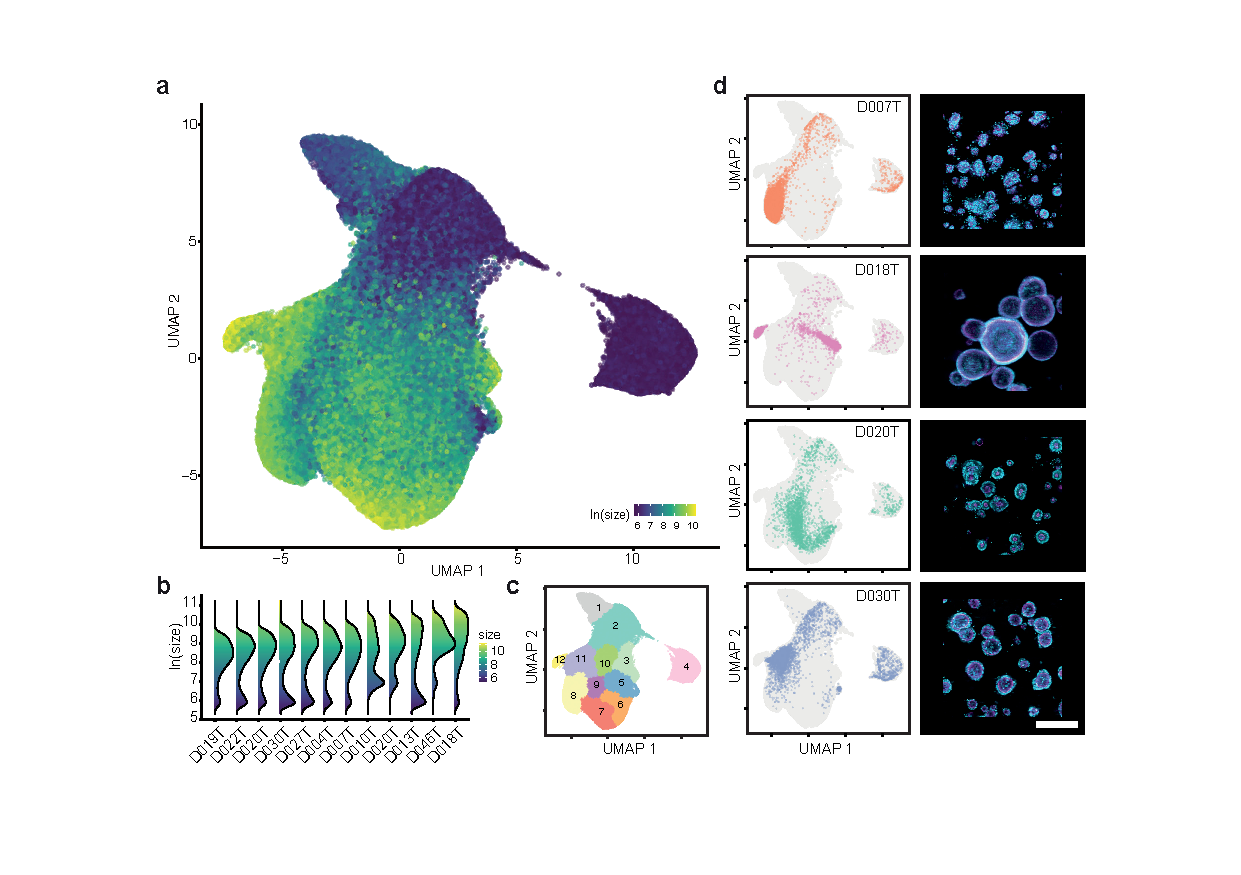
\includegraphics[width=\textwidth,
                height=\textheight,
                keepaspectratio]{figures/promise/pdf/fig_1_4.pdf}
\caption[Image-based profiling captures the phenotype diversity of patient derived cancer organoids]{\textbf{Image-based profiling captures the phenotype diversity of patient derived cancer organoids a} Uniform Manifold Approximation and Projection (UMAP) of 25 morphology principal components at single-organoid-resolution for a random 5\% sample out of ca. 5.5 million organoids. The same sample is used for visualizations throughout the figure. Color corresponds to the log-scaled organoid area (dark blue: minimum size, yellow: maximum size). \textbf{b} organoid size distribution across lines. \textbf{c} UMAP representation of DMSO treated and drug treated organoids. Graph-based clustering of organoids by morphology. \textbf{d} UMAP embeddings of selected organoid lines (baseline state / 0.1\% DMSO control-treated organoids) representing different morphological subsets, grey background consists of randomly sampled points. Depicted are representative example images for each line (right, cyan = DNA, magenta = Actin, scale-bar: 200µm). Figure adapted from \textit{The drug-induced phenotypic landscape of colorectal cancer organoids} \parencite{betgeDruginducedPhenotypicLandscape2022}. Johannes Betge retrieved the example images for part d.}
\label{fig_140}
\end{figure}
\bigbreak

To visualize the heterogeneity of colorectal cancer organoids and drug induced changes across and within cancer organoid lines, the 25 principal components of  ca. 5.5 million profiled organoids were embedded using uniform manifold approximation and projection (UMAP) (Figure \ref{fig_140} a and \ref{fig_145} a-c). Most organoid lines showed characteristic bimodal log-normal distributions of organoid size with one component containing small organoids and another component made up of larger organoids with varying, line specific, average size (Figure \ref{fig_140} b, and \ref{fig_145} d-e). The log-normal-like size distribution likely resulted from intrinsic differences in cellular size and growth rate compounding over time in multicellular organoids. 

\bigbreak
While DNA and Actin staining intensity were positively correlated with organoid size, cell permeability was negatively correlated and enriched in regions with relatively smaller organoids (Figure \ref{fig_145} a-c). Graph-based clustering of this identified 12 regions within the embedding (Figure \ref{fig_140} c). When comparing drug-treated organoids to organoids treated with the negative control (DMSO), no clear separation of these two groups, except an increased presence of drug-treated organoids in region 3,  was seen. This finding suggested that organoid morphology was distributed on a continuum of phenotypes spanning perturbed and unperturbed conditions of the experiment (Figure \ref{fig_145} f). 
\bigbreak

Different organoid lines within the embedding were located in characteristic regions, with organoid size and organoid architecture as primary organizing factors (Figure \ref{fig_140} b and d). For example, organoid line D018T had the largest median organoid size within the dataset and a cystic organoid architecture, while D020T organoids had a solid architecture and smaller median size. In most cases, organoid lines had two areas of main density, with one of them in regions 2, 3 or 4, reflecting the previously mentioned bimodal size distribution. In summary, image-based profiling of patient derived colorectal cancer organoids showed strong morphological heterogeneity with line dependent differences in size and organoid architecture.

\begin{figure}[h]
\centering
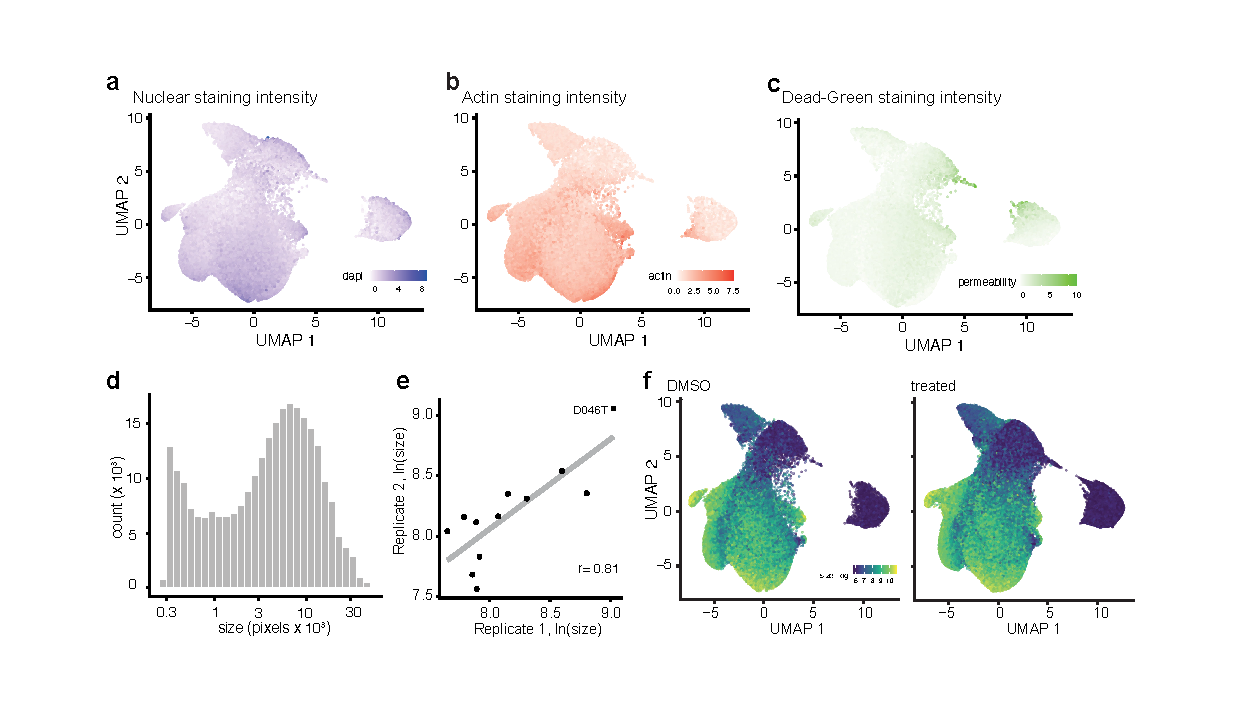
\includegraphics[width=\textwidth,
                height=\textheight,
                keepaspectratio]{figures/promise/pdf/fig_1_5.pdf}
\caption[Basic image-based features and their role in organoid phenotype diversity]{\textbf{Basic image-based features and their role in organoid phenotype diversity. a-c} Uniform Manifold Approximation and Projection (UMAP) of organoid-level features marked by DNA (DAPI) staining intensity (b), actin (Phalloidi/FITC) staining intensity (c) and permeability (Image-IT DeadGreen) staining intensity \textbf{d} Distribution of organoid size for all control (DMSO) treated organoids. \textbf{e} Replicate correlation of organoid size for control treated organoids. \textbf{f} UMAP representation of DMSO treated and drug treated organoids. Figure adapted from \textit{The drug-induced phenotypic landscape of colorectal cancer organoids} \parencite{betgeDruginducedPhenotypicLandscape2022}}
\label{fig_145}
\end{figure}
\bigbreak

Exploratory data analysis of the relationship between organoid morphology and experimental batch showed overall reproducible measurements of organoid size across experiments (Figure \ref{fig_145} e). Similarly, further analysis of the UMAP showed overlapping morphology distributions between replicates for a given organoid line (Figure \ref{fig_216} a). Given that line differences were confounded by experimental batches (experimental batches and tested organoid lines were not independent), no procedure to reduce possible batch-dependent differences in organoid phenotype were performed. 

\bigbreak

\begin{figure}[!h]
\centering
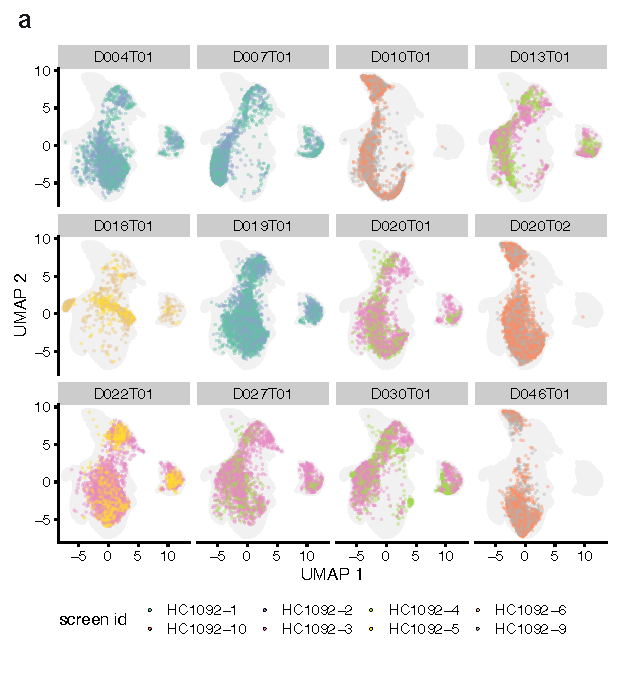
\includegraphics[width=250pt,
                height=\textheight,
                keepaspectratio]{figures/promise/pdf/fig_1_6.pdf}
\caption[Experimental batches and their impact on organoid phenotype]{\textbf{Experimental batches and their impact on organoid phenotype. a} UMAP of organoid level features stratified by organoid line and colored by experimental batch.}
\label{fig_216}
\end{figure}


\subsection{Organoid phenotype-profiles capture organoid viability}

Cell viability assays are common readouts in cancer drug discovery. Prompted by the observation that organoid size was a major factor determining the structure of the phenotype embedding (UMAP and factor 1 in MOFA analysis, see below), I hypothesized that low organoid size was at least partially the result of cell death within the organoid and, more broadly, that phenotype data could be used to estimate organoid viability. Bortezomib, a small molecule proteasome inhibitor with high \textit{in-vitro} toxicity led to dose dependent organoid death in all organoid lines, thus representing suitable positive controls (Figure \ref{fig_221} a). Analogous to pseudotime in single-cell  gene expression analysis, dose-dependent trajectories of Bortezomib drug response could be fitted (Figure \ref{fig_221} b) using the non-parametric principle curve method. Starting from diverse baseline morphologies, increasing doses of Bortezomib led to a step-wise convergence on a final death-related phenotype, which corresponded to the areas with enrichment of small objects (regions 2, 3 and 4). 

\begin{figure}[h]
\centering
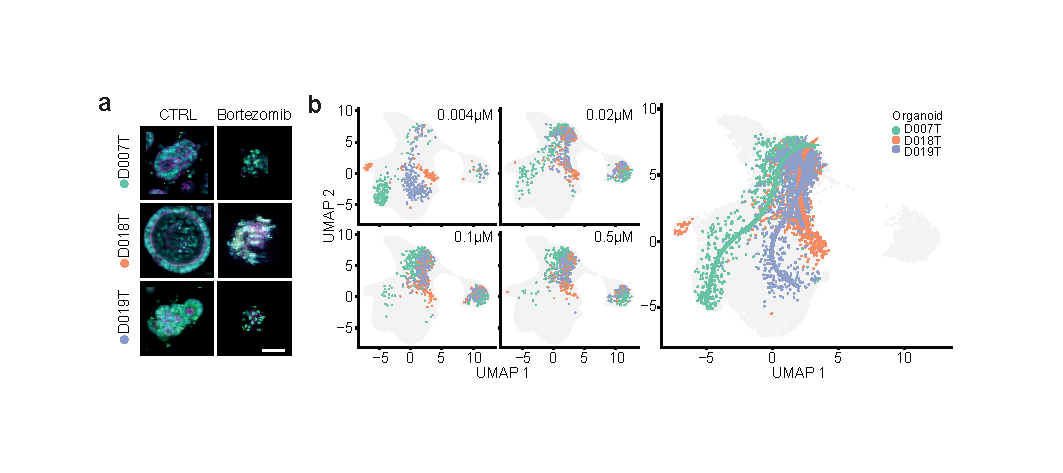
\includegraphics[width=\textwidth,
                height=\textheight,
                keepaspectratio]{figures/promise/pdf/fig_2_1.pdf}
\caption[Organoid phenotype-profiles capture organoid viability]{\textbf{Organoid phenotype-profiles capture organoid viability. a} Representative example images of negative- (0.1\% DMSO) and positive control treated organoids (2.5µM bortezomib, cyan = DNA, magenta = actin, yellow = cell permeability; average images were selected and embedded in black background; scale bar: 50µm). b, Dose-dependent-trajectory of bortezomib treatment effect. UMAP of organoid morphology at different bortezomib doses and (right panel) dose-dependent trajectory for three representative organoid lines. For visual purposes, trajectory inference was limited to partition 1, the left-hand set of measurements within the UMAP, representing ca. 95 \% of all imaging data. Panel a created with support from Johannes Betge. Figure adapted from \textit{The drug-induced phenotypic landscape of colorectal cancer organoids} \parencite{betgeDruginducedPhenotypicLandscape2022}. Johannes Betge retrieved the example images for part a.}
\label{fig_221}
\end{figure}
\bigbreak

Similarly, Paclitaxel, a microtubule disassembly inhibitor, shifted the bimodal size distribution of organoids in a dose-dependent fashion (Figure \ref{fig_222} a), while organoid count remained largely unchanged (Figure \ref{fig_222} b). This effect, however, was organoid line-specific, as median organoid size in Paclitaxel sensitive lines (e.g. D022T) decreased, while the size of other organoids remained unaffected (e.g. D046T, Figure \ref{fig_222} c-f). These observations suggested a link between organoid morphology, especially organoid size, with a loss of cell viability. 

\bigbreak
To further test the link between organoid morphology and cell viability, a luminescence-based, ATP dependent, cell viability assays (CTG) was performed in parallel with imaging as benchmark. A correlation of CTG viability with organoid size (r = 0.64) (Figure \ref{fig_223} a) was visible. Organoid size showed the most robust correlation with luminescence-based viability measurements across all profiled organoid lines (Figure \ref{fig_223} b), while other features, such as DAPI, Actin, and membrane permeability (DeadGreen) intensity were less suitable to predict the viability of organoids. In conclusion, organoid size is an informative metric to approximate organoid viability, but is biased by line-specific differences in organoid size.


\begin{figure}[h]
\centering
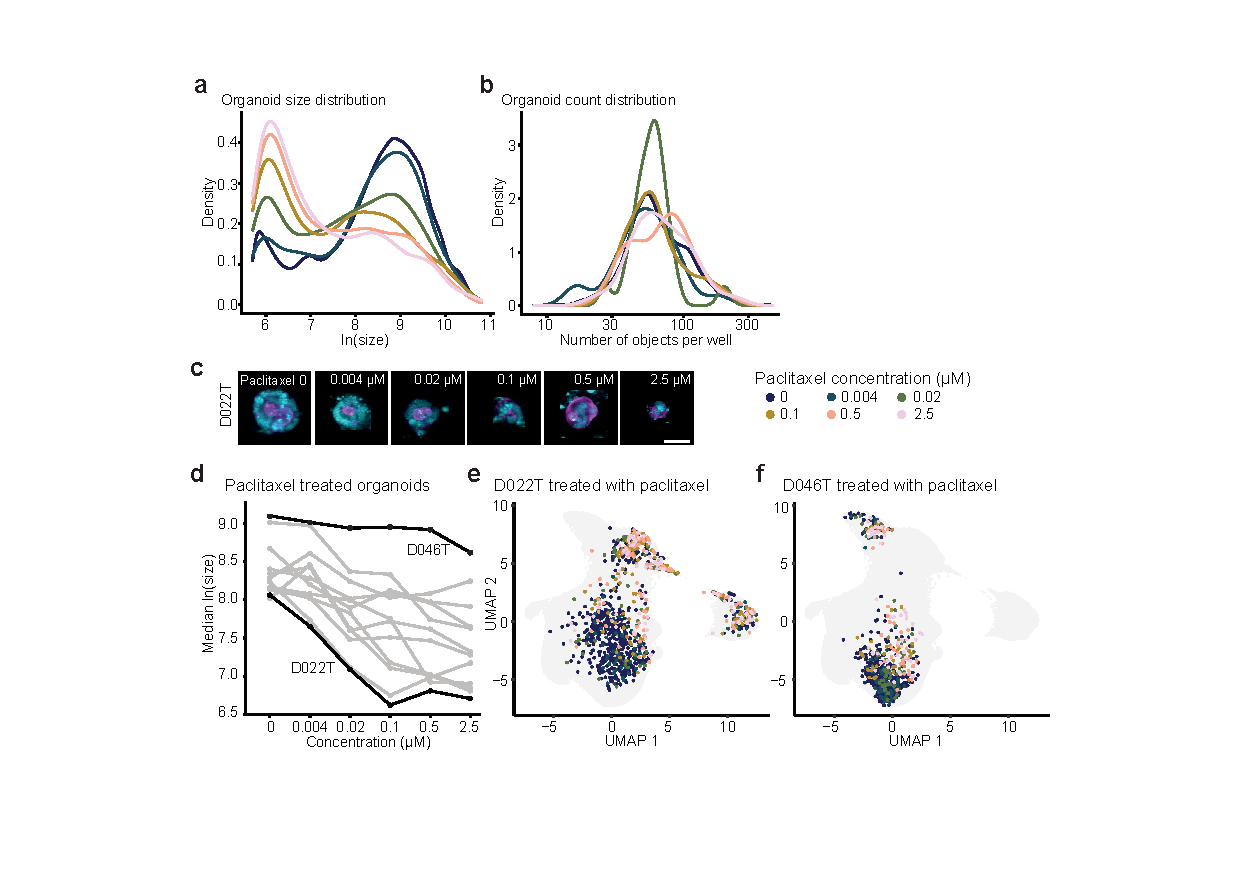
\includegraphics[width=\textwidth,
                height=\textheight,
                keepaspectratio]{figures/promise/pdf/fig_2_2.pdf}
\caption[Organoid phenotype-profiles capture treatment specific changes in organoid viability]{\textbf{Organoid phenotype-profiles capture treatment specific changes in organoid viability. a} Distribution of organoid size at different concentrations of Paclitaxel. Shown is a random sample of 30\% of all Paclitaxel treated organoids for this and following figures. \textbf{b} Distribution of organoid number per well at different concentrations of Paclitaxel. \textbf{c} Example images of D022T organoids treated with Paclitaxel. \textbf{d} Dose-response relationship of organoid size and paclitaxel dose. D022T and D046T are highlighted. \textbf{e} UMAP of organoid morphology highlighting D022T organoids treated at different concentrations of Paclitaxel. \textbf{f} UMAP of organoid morphology highlighting D046T organoids treated at different concentrations of Paclitaxel. Figure adapted from \textit{The drug-induced phenotypic landscape of colorectal cancer organoids} \parencite{betgeDruginducedPhenotypicLandscape2022}. Johannes Betge retrieved the example images for part c.}
\label{fig_222}
\end{figure}
\bigbreak


\clearpage
\begin{figure}[h]
\centering
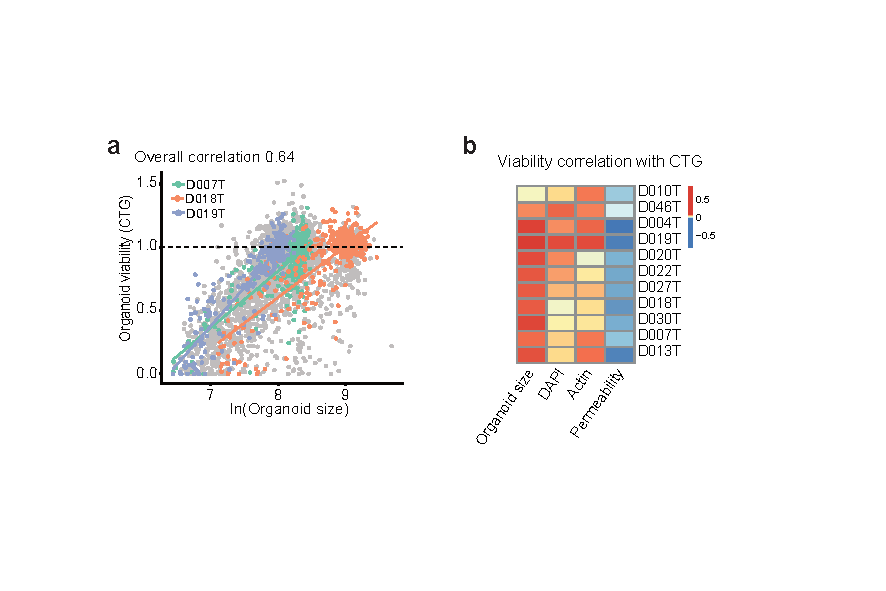
\includegraphics[width=\textwidth,
                height=\textheight,
                keepaspectratio]{figures/promise/pdf/fig_2_3_2.pdf}
\caption[Organoid phenotype-profiles reflect ATP-dependent viability measurements]{\textbf{Organoid phenotype-profiles reflect ATP-dependent viability measurements. a} Association of organoid size of selected example lines with organoid viability determined by luminescence-based, ATP-dependent viability profiling with CellTiter-Glo (CTG), which was performed in parallel with imaging on a subset of drug treatments. \textbf{b} Association of Organoid size and representative features (DNA, actin and permeability dye intensities) with benchmark CTG viability read out. Figure adapted from \textit{The drug-induced phenotypic landscape of colorectal cancer organoids} \parencite{betgeDruginducedPhenotypicLandscape2022}}
\label{fig_223}
\end{figure}
\bigbreak

\subsection{Drug induced organoid phenotypes correspond to drug mechanism of action}

An advantage of image-based profiling over one-dimensional cell viability measurements in drug discovery is the ability to use the high dimensional drug-induced phenotype-profiles to identify small molecule mechanism of action based on similarity towards other, well-annotated, small molecules. 

\begin{figure}[!h]
\centering
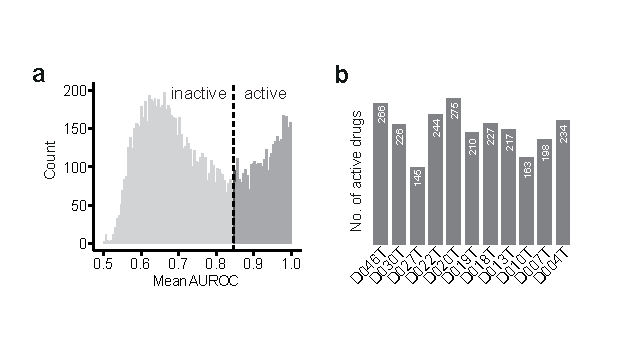
\includegraphics[width=300pt,
                height=\textheight,
                keepaspectratio]{figures/promise/pdf/fig_3_0_1.pdf}
\caption[Distribution of AUROC drug activity scores]{\textbf{Distribution of AUROC drug activity scores. a} Distribution of AUROC scores across all studied organoid models and treatments. \textbf{b} Number of active treatments per organoid line. Figure adapted from \textit{The drug-induced phenotypic landscape of colorectal cancer organoids} \parencite{betgeDruginducedPhenotypicLandscape2022}. Analysis was performed by Jan Sauer.}
\label{fig_230}
\end{figure}
\bigbreak

To test whether this approach could be used in cancer organoids, a weakly supervised learning approach to identify treatment effect vectors was developed with the support of Jan Sauer. Briefly, for every treatment and genotype, a logistic regression classifier was trained to distinguish DMSO-treated organoids from small molecule treated organoids. The resulting normal vector between control- and treated organoid profiles was referred to as the treatment effect vector. The classification performance, expressed as the AUROC, was used to determine the activity of a treatment, where the activity was defined  (AUROC, mean from bootstrapped modeling with values ranging from 0.5 to 1). A high AUROC score (approaching 1) is observed for compounds that lead to a treatment-induced organoid morphology that is highly distinct from DMSO treated organoids. In contrast a low AUROC (centered around 0.5) is observed for compounds where the model's classification performance approaches random guessing (Figure \ref{fig_230} a, b). I referred to the AUROC as the drug activity score. To test whether active drugs systematically lead to organoid phenotypes that are informative of mechanism of action, the cosine distance between concatenated treatment effect vectors was determined. This approach led to a clustering of specific mode-of-actions, including inhibitors of MEK, Aurora kinase, CDK, mTOR, AKT, EGFR or GSK3-beta (Figure \ref{fig_231} a). 
\bigbreak

Compounds with related, but not identical, targets also induced related phenotypes, for example MEK inhibitors clustered with specific RAF- and ERK inhibitors (Figure \ref{fig_231} c-f) or AKT and PI3K inhibitors were part of a cluster mainly containing mTOR targeting compounds. Manual inspection of several phenotypes (Figure \ref{fig_231} g) revealed characteristic treatment-induced phenotypes. Most notably, MEK inhibitors led to reorganization towards more cystic organoid architecture. These target dependent phenotypes were observable across organoid lines and drugs.

\begin{figure}[H]
\centering
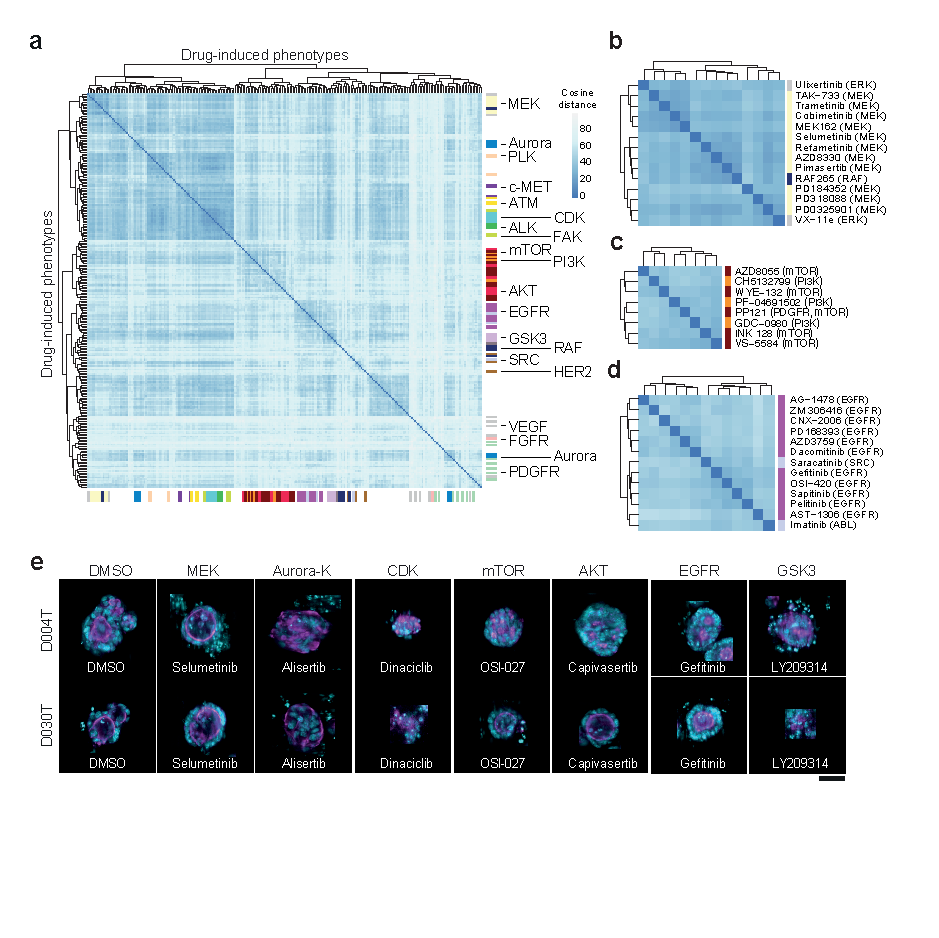
\includegraphics[width=\textwidth,
                height=\textheight,
                keepaspectratio]{figures/promise/pdf/fig_3_1_1.pdf}
\caption[Clustering of treatment effects captures mechanism of action]{\textbf{Clustering of treatment effects captures mechanism of action. a} Hierarchical clustering of treatment effect vectors across all observed organoid models. Clustering is based on the cosine distance of concatenated treatment effect vectors. Sidebars are color-coded by the primary annotated target. \textbf{b-d} Magnified regions from panel a showing clusters of small molecule inhibitors targeting MEK, mTOR, and EGFR. \textbf{e} Representative images of treatment-induced organoid phenotypes for seven clusters of small molecules (cyan = DNA, magenta = actin, yellow = cell permeability; average images were selected and embedded in black background; scale bar: 50µm). Figure adapted from \textit{The drug-induced phenotypic landscape of colorectal cancer organoids} \parencite{betgeDruginducedPhenotypicLandscape2022}. Analysis was performed by Jan Sauer and retrieval of example images in part e was done in collaboration with Johannes Betge.}
\label{fig_231}
\end{figure}
\bigbreak

To validated the previous results with a second analysis approach, alternative methods to 1) quantify treatment activity and 2) cluster treatment effects by similarity were evaluated. The AUROC score which was previously used to define active treatments, correlated with the euclidean distance of phenotype profiles (Spearman Correlation = 0.91). Similarly, evaluating an alternative clustering method based on phenotype profile averaging across lines (instead of concatenating) followed by clustering recovered an overall similar grouping of treatments (Figure \ref{fig_232} a). 

\begin{figure}[H]
\centering
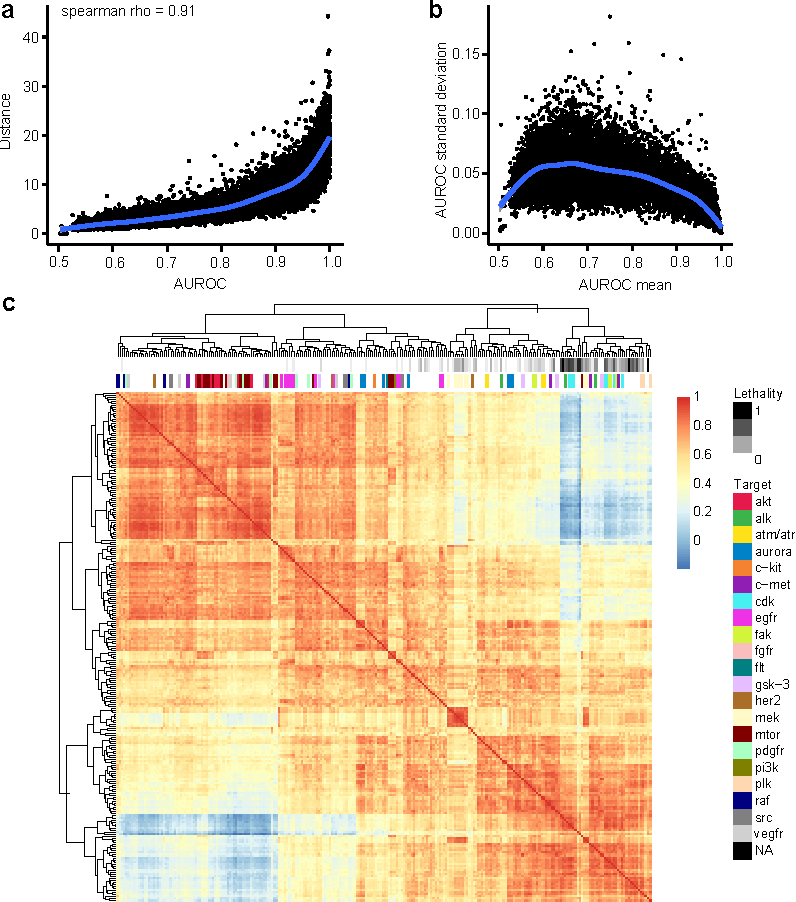
\includegraphics[width=\textwidth,
                height=\textheight,
                keepaspectratio]{figures/promise/pdf/fig_3_2.pdf}
\caption[Validation of treatment activity and effect quantification method]{\textbf{Validation of treatment activity and effect quantification method. a} Hierarchical clustering of treatment effect vectors across all observed organoid models. Clustering is based on the euclidean distance of average treatment effect vectors. Sidebars are color-coded by the primary annotated target.}
\label{fig_232}
\end{figure}
\bigbreak

\newpage

\section{Multi-omics factor analysis identifies factors linking morphology, genomic data and drug activity}

A limitation of image-based profiling experiments is that both unperturbed and treatment-induced phenotypes are challenging to interpret. I hypothesized that, in the presence of multiple \textit{in-vitro} models with both phenotype and transcriptome measurements, links between the two data modalities can be learned. 

\begin{figure}[!h]
\centering
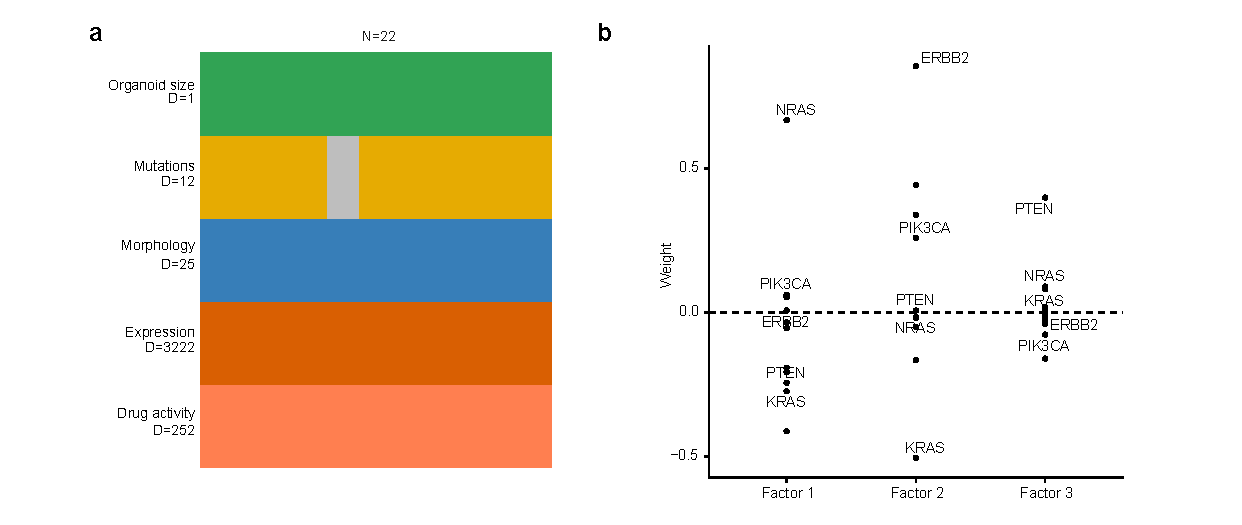
\includegraphics[width=280pt,
                height=\textheight,
                keepaspectratio]{figures/promise/pdf/fig_4_2.pdf}
\caption[Overview of input data for MOFA modeling]{\textbf{Overview of input data for MOFA modeling. a} 22 observations of 11 models across 5 different views (size, mutation, morphology, gene expression and treatment activity) were integrated in the model. Missing data is shown in grey. "D" represents the vector length of the respective view. Figure adapted from \textit{The drug-induced phenotypic landscape of colorectal cancer organoids} \parencite{betgeDruginducedPhenotypicLandscape2022}.}
\label{fig_242}
\end{figure}

To learn a multi-view representation of unperturbed organoid morphology, unperturbed organoid size, transcript expression, somatic mutations, and drug activity, multi-omics factor analysis (MOFA) was performed. MOFA is a matrix factorization method built upon group factor analysis, with decomposes a set of different measurements into a shared matrix of factor scores for each observed sample and a set of corresponding matrices linking each factor to features in the set of original measurements through a weight or "loading" \parencite{argelaguetMultiOmicsFactorAnalysis2018b}. 

\subsection{Learning a multi-view representation with MOFA}

The support data used to fit the MOFA model consisted of a set of five matrices, each with 22 observations (rows) representing 11 organoid models with 2 replicates per model (Figure \ref{fig_241} a). Each matrix represented a modality (mutation, morphology, gene expression, etc.). When trained with a low number of k = 3 factors, MOFA recovered factors explaining between ca. 41 and 24\% of variance across the different data modalities, with the first two factors accounting for on average ca. 29 and 17\% in aggregate, respectively (Figure \ref{fig_240} a). While gene expression, mutations and drug activity profiles for organoid lines contributed to all factors, factor 1 captured an exceptional amount of variation in median organoid size (ca. 39\%). In contrast, factor 2 was primarily capturing variation within baseline organoid morphology (ca. 16\%) (Figure \ref{fig_240} a).

\begin{figure}[!h]
\centering
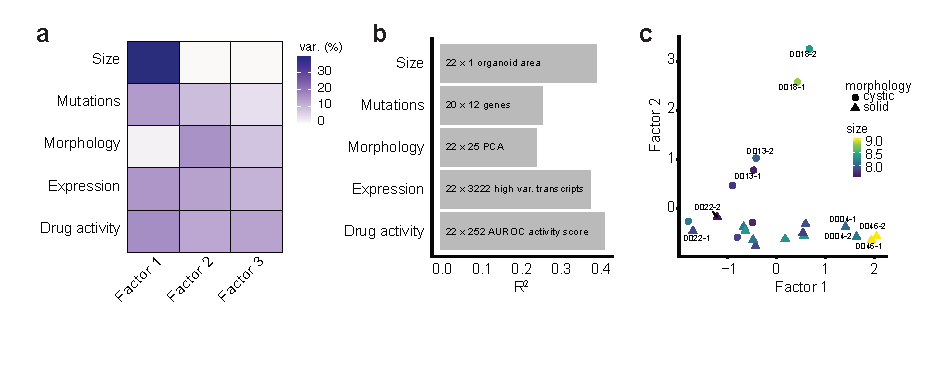
\includegraphics[width=\textwidth,
                height=\textheight,
                keepaspectratio]{figures/promise/pdf/fig_4_0.pdf}
\caption[Mulit-omics factor analysis of organoid profiles]{\textbf{Mulit-omics factor analysis of organoid profiles. a-b} Variance decomposition of the MOFA model. Shown is the variance explained for every factor and data modality, as well as only by modality. \textbf{c} Factor scores for individual observations. The shapes represent the manually determined morphology label and color average organoid size. Figure adapted from \textit{The drug-induced phenotypic landscape of colorectal cancer organoids} \parencite{betgeDruginducedPhenotypicLandscape2022}.}
\label{fig_240}
\end{figure}
\bigbreak

Overall, MOFA factors explained up to 40\% of variance in median organoid size, drug activity and transcript expression, while less than 30\% of variance in baseline organoid morphology was explained by the model (Figure \ref{fig_240} b). Organoid lines D046T and D004T stood out as lines with the strongest score for factor 1, while lines D018T and D013T had the strongest score in factor 2. Visual inspection of organoids revealed that organoid lines with a higher factor 1 score tended to be larger in size and organoids with high factor 2 score tended to have a more cystic organoid architecture based on manual classification (Figure \ref{fig_240} c). No interpretable morphological differences between factor 3 low and high organoids were identifiable, so the subsequent analysis was focused on the first two interpretable factors generated by MOFA. 
\bigbreak

To validate the MOFA finding and evaluate whether morphological differences could be seen in transcript expression data directly, I visualised organoid models by a set of previously determine manual morphology labels (Figure \ref{fig_241} a) and measured size (Figure \ref{fig_241} b) in a principal component analysis. The transcript expression data alone organised patient derived organoid models by their manual morphology labels. To summarize, unsupervised multi-view representation learning with MOFA identified factors within the dataset that explained variation between organoid lines across different data modalities, including organoid morphology and median organoid size.

\begin{figure}[!h]
\centering
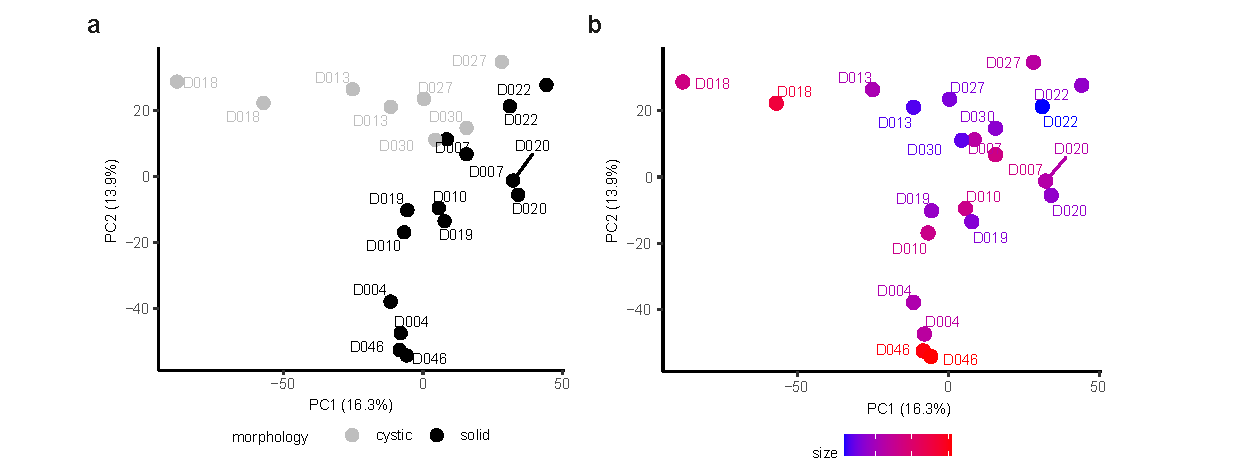
\includegraphics[width=500pt,
                height=\textheight,
                keepaspectratio]{figures/promise/pdf/fig_4_1.pdf}
\caption[Validation of characteristic organoid phenotypes by transcript expression analysis]{\textbf{Validation of characteristic organoid phenotypes by transcript expression analysis. a} PCA of transcript expression data for organoid models. Observations are color-coded by the manually determined morphology label. \textbf{b} Identical PCA of transcript expression data, color-coded by average organoid size.}
\label{fig_241}
\end{figure}


\newpage
\subsection{An IGF1R signaling program is associated with increased organoid size, EGFR inhibitor resistance and can be induced by mTOR inhibition}

Differences in organoid size are a contributing factor to intra- and inter-organoid line heterogeneity. Organoid size was influenced by both organoid line and drug treatments and was associated with factor 1 scores (Figure \ref{fig_261} a). An unsupervised gene set enrichment analysis (GSEA) for Reactome pathways across factor 1 loadings showed an enrichment for IGF1R signaling and mitogen-activated protein kinase signaling related genes (Figure \ref{fig_261} b). 

\begin{figure}[h!]
\centering
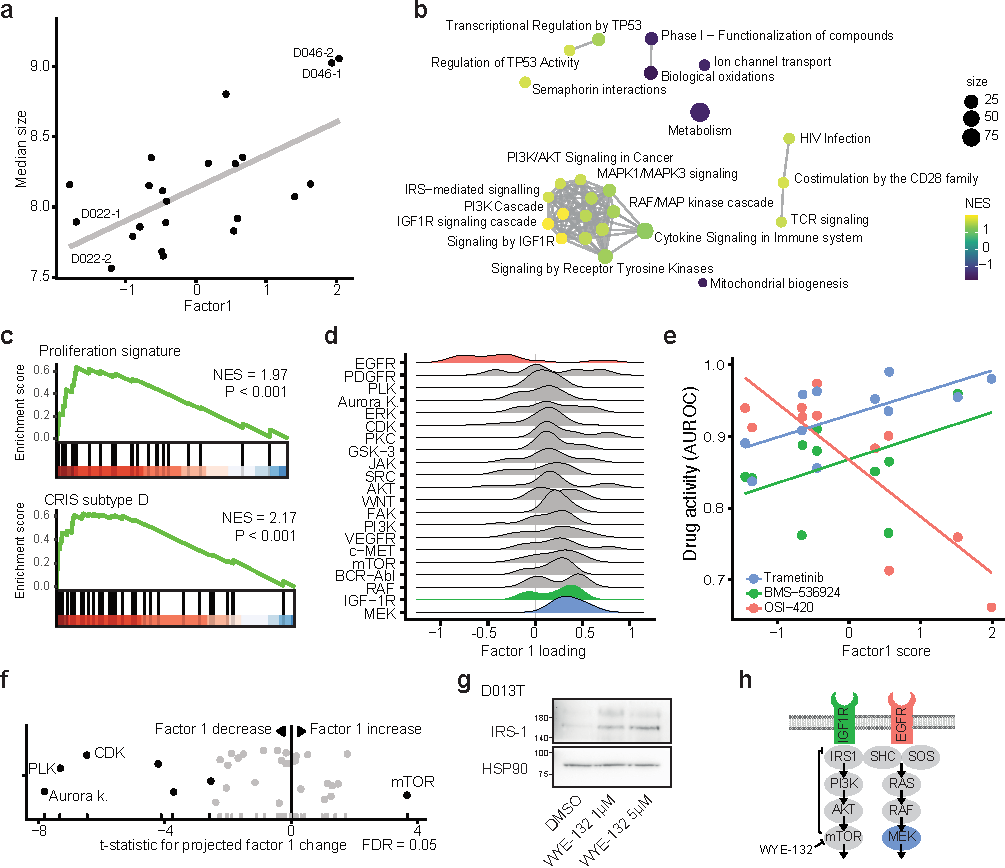
\includegraphics[width=\textwidth,
                height=\textheight,
                keepaspectratio]{figures/promise/pdf/fig_6_1.pdf}
\caption[Factor 1 overview]{\textbf{Factor 1 overview. a} Association between organoid size and factor 1 score. \textbf{b} GSEA network of factor 1 gene expression loadings. An edge connects Reactome pathways with more than 20\% overlap. \textbf{c} GSEA of the proliferation signature and the colorectal cancer CRIS-D subtype over ranked factor 1 gene expression loadings (ranking from high factor 1 to low factor 1 loading). \textbf{d} Distributions of treatment activity score loadings grouped by targets for factor 1. \textbf{e} Relationship of selected treatment activity scores (AUROC) with factor 1 score. \textbf{f} Projection of factor 1 scores for drug-induced phenotypes. Highlighted are drug targets leading to a significant change in projected factor scores across all organoid lines (ANOVA). \textbf{g} Western blot of IRS-1 protein abundance under mTOR inhibition for a representative organoid line (D013T). \textbf{h} Illustration of IGF1R signaling pathway with highlighted drug targets. Shown is the disinhibition of mTOR mediated IRS-1 repression after treatment with mTOR inhibitors. Figure adapted from \textit{The drug-induced phenotypic landscape of colorectal cancer organoids} \parencite{betgeDruginducedPhenotypicLandscape2022}. Validating Western Blot and visual summary in parts g and h were contributed by Johannes Betge.}
\label{fig_261}
\end{figure}
\bigbreak

In fact, the IGF signaling related transcripts H19 (rank 1) and IGF2 (rank 13) were among the strongest contributors to factor 1. This increase in proliferative signaling was confirmed by GSEA of a previously identified intestinal proliferation signature by Merlos-Suarez et al. \parencite{merlos-suarezIntestinalStemCell2011} (Figure \ref{fig_261} c). To better understand clinical correlates to the identified gene expression patterns, I tested for an enrichment of molecular subtype profiles stemming from an analysis of cancer-cell intrinsic transcription \parencite{isellaSelectiveAnalysisCancercell2017}. Factor 1 showed an enrichment for CRIS D, a molecular subtype linked to IGF2 overexpressing tumors, loss of IGF2 imprinting and resistance to EGFR inhibitor therapy (Figure \ref{fig_261} c). Conversely, I observed a depletion for CRIS C, which has been linked to EGFR dependency (Figure \ref{fig_262} a and b). In fact, activity of EGFR inhibitors was the strongest contributor to a negative factor 1 score while IGF1R and MEK inhibitor activity contributed to a positive factor 1 score (Figure \ref{fig_261} d-e and Figure \ref{fig_262} c-e).

\begin{figure}[h!]
\centering
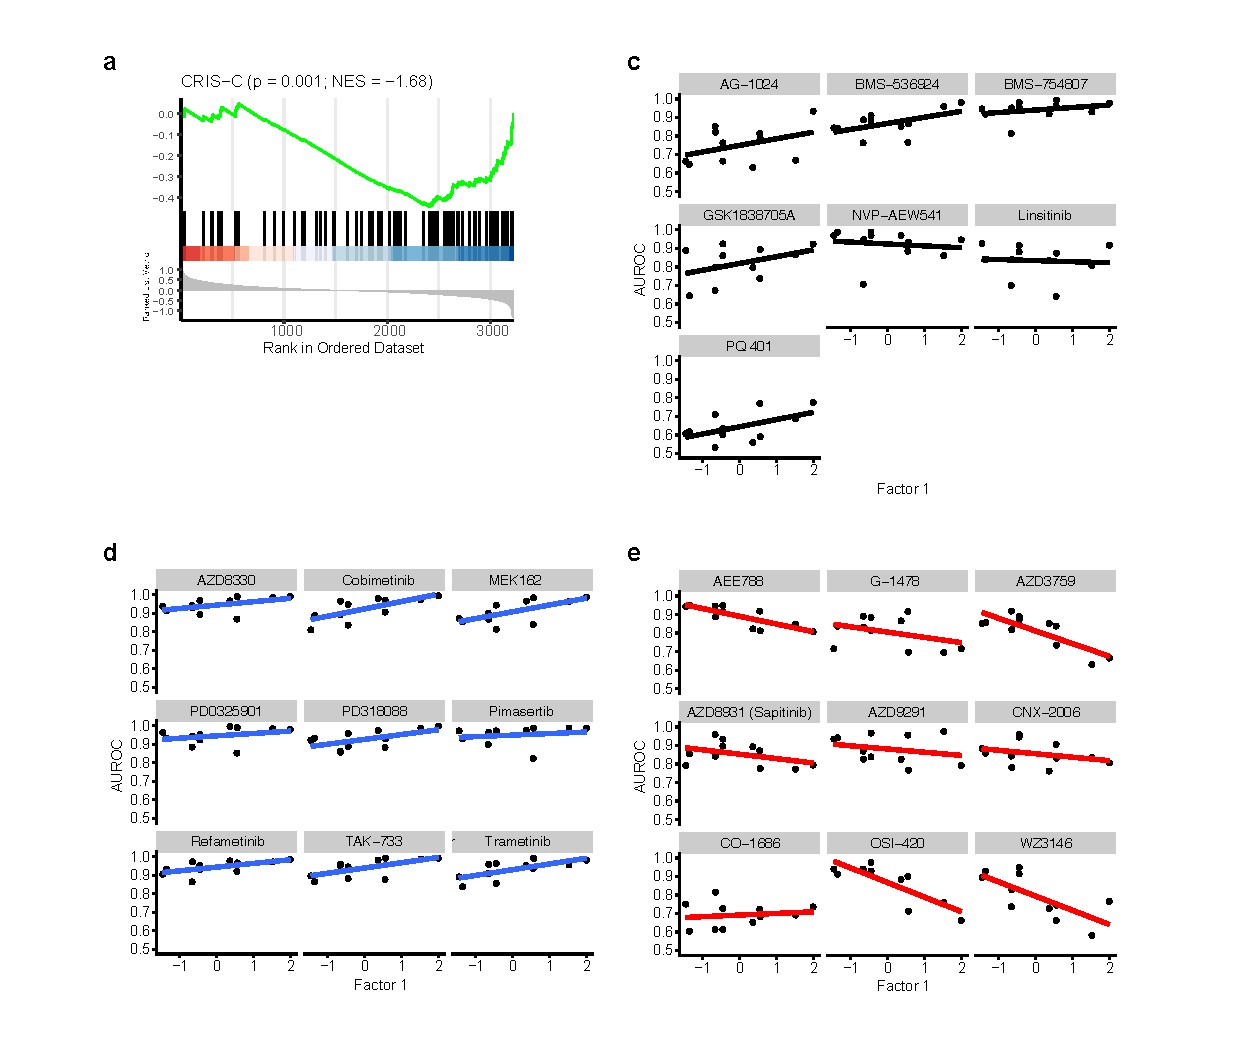
\includegraphics[width=\textwidth,
                height=\textheight,
                keepaspectratio]{figures/promise/pdf/fig_6_2_1.pdf}
\caption[Factor 1 extended overview]{\textbf{Factor 1 extended overview. a} GSEA of the CRIS C subtype signature over ranked factor 1 gene expression loadings. \textbf{b-d} Association between treatment activity scores and factor 1 scores for three classes of compounds, targeting IGF1R, MEK and EGFR, respectively. Figure adapted from \textit{The drug-induced phenotypic landscape of colorectal cancer organoids} \parencite{betgeDruginducedPhenotypicLandscape2022}.}
\label{fig_262}
\end{figure}
\bigbreak

To test whether small molecule treatments shifted organoids in factor space, the morphological features of treated organoids set were projected into factor space. This projection was performed using the pseudoinverse of the loading matrix and multiplying it with the treatment-induced morphology features for treatments of interest. This approach enables interpreting treatment-induced phenotypes in a representation space that was previously learnt from multi-view data of unperturbed organoids. 

\bigbreak
A group of cell cycle related kinase inhibitors targeting polo like kinases, Aurora kinases and cyclin dependent kinases shifted organoids to a low factor 1 score (Figure \ref{fig_261} f). In contrast, mTOR inhibitor treatment increased factor 1 scores in cancer organoids (Figure \ref{fig_261} f). Given the observation that factor 1 was associated with IGF-1R signaling and mTOR inhibitor treatment led to an increase in factor 1 scores, I hypothesized that mTOR inhibition leads to a reactive upregulation of IGF1R signaling in cancer organoids. In fact, inhibition of mTOR signaling had previously been linked to transcriptional disinhibition of IRS-1 in a negative feedback loop \parencite{oreillyMTORInhibitionInduces2006} and  reactive induction of IGF1R signaling had previously been described as a resistance mechanism to small molecule mTOR inhibitors in cancer \parencite{sharmaChromatinmediatedReversibleDrugtolerant2010}. When testing this hypothesis in patient derived organoids, a dose-dependent increase of IRS-1 protein abundance in organoids treated with the ATP competitive mTOR inhibitor WYE-132 was observable (Figure \ref{fig_261} g and h). 

\bigbreak
To summarize, factor 1 described an organoid state with increased organoid size, elevated IGF1R dependent mitogenic signaling and increased resistance to EGFR inhibitors. This state could be induced by inhibiting mTOR, leading to a disinhibition of a negative feedback loop controlling IGF1R signaling.

\newpage
\subsection{An LGR5+ program is associated with cystic organoid architecture, Wnt signaling inhibitor sensitivity, and can be induced by inhibition of MEK}

Besides size differences, a particularly strong recurring organoid phenotype was the presence of a cystic organoid architecture, seen for example in untreated D018T organoids and organoids treated with MEK inhibitors (Figure \ref{fig_140} and \ref{fig_231}). In the cystic state, which was observed in factor 2 high organoid lines (i.e. D018T), organoids consisted of a monolayer of uniform cells lining a central spherical lumen with a distinct apico-basally oriented actin cytoskeleton (Figure \ref{fig_251} a and b). This phenotype was reminiscent of organoid morphologies previously seen in \textit{APC}textsuperscript{-/-} or Wnt ligand treated human intestinal organoids \parencite{matanoModelingColorectalCancer2015a}. 

\begin{figure}[h!]
\centering
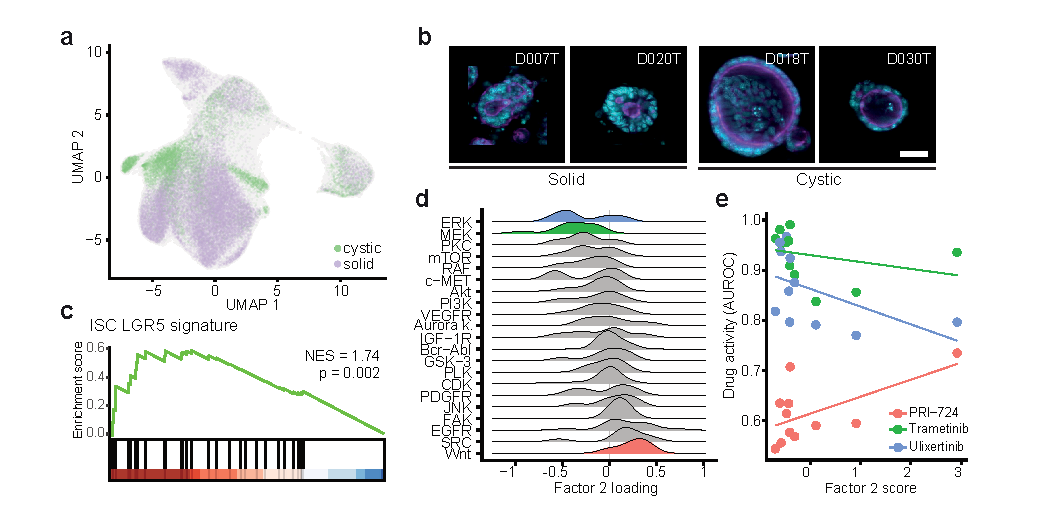
\includegraphics[width=\textwidth,
                height=\textheight,
                keepaspectratio]{figures/promise/pdf/fig_5_1.pdf}
\caption[Factor 2 overview]{\textbf{Factor 2 overview. a} UMAP of observed organoids. Color labels represent the manually determined morphology labels. \textbf{b} Representative images of solid and cystic organoid phenotypes (cyan = DNA, magenta = actin, yellow = cell permeability; average images were selected and embedded in black background; scale bar: 50µm). \textbf{c} GSEA of LGR5 gene expression signature over ranked factor 2 gene expression loadings (ranking from high factor 2 to low factor 2 loading). \textbf{d} Distributions of treatment activity score loadings grouped by targets for factor 2. \textbf{e} Relationship of selected treatment activity scores (AUROC) with factor 2 score. Example images curated with support from Johannes Betge. Figure adapted from \textit{The drug-induced phenotypic landscape of colorectal cancer organoids} \parencite{betgeDruginducedPhenotypicLandscape2022}. Johannes Betge retrieved the example images for part b.}
\label{fig_251}
\end{figure}
\bigbreak

To test if factor 2 comprised Wnt signaling and intestinal stem cell identity related gene expression programs, gene set enrichment analyses (GSEA) was performed for cell identity signatures previously described by Merlos-Suarez et al. \parencite{merlos-suarezIntestinalStemCell2011}. GSEA revealed an enrichment of Lgr5+ stem cell signature-related genes for the factor 2 loadings (FDR=0.002, NES=1.74) (Figure \ref{fig_251} c). Activity of Wnt signaling inhibitors and EGFR inhibitors were the strongest average contributors to a positive factor 2 score (t statistic = 3.02, FDR = 0.046 and t statistic = 3.08, FDR = 0.046, respectively), while activity of ERK and MEK inhibitors were associated with a low factor 2 score (Figure \ref{fig_251} d), albeit not significantly. As expected from these results, factor 2 high organoid lines showed a stronger morphological response to the Wnt pathway inhibitor PRI-724. (Figure \ref{fig_251} e).

\begin{figure}[h!]
\centering
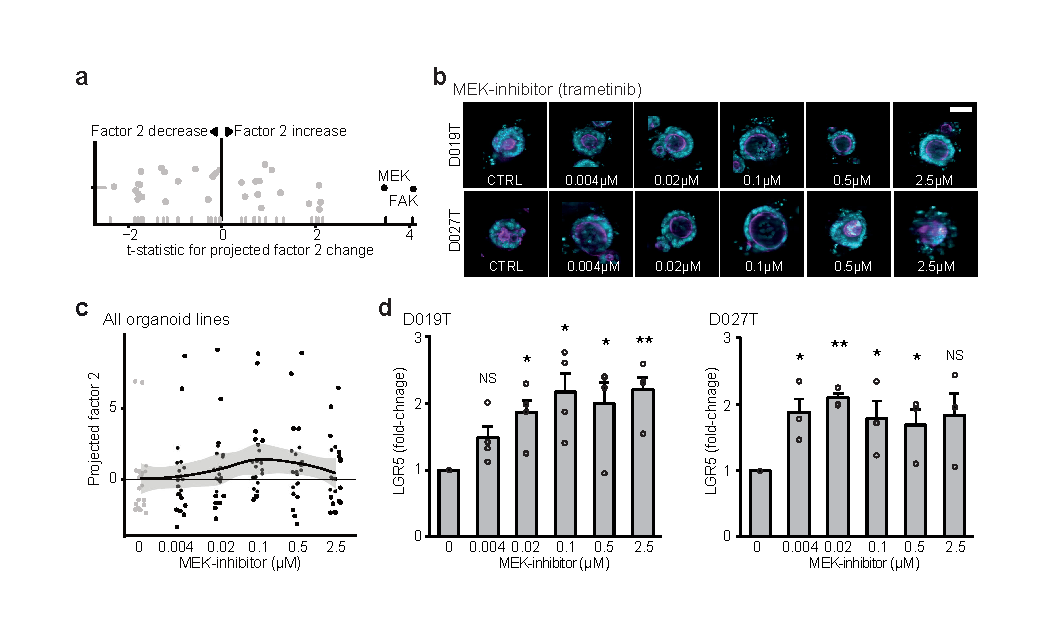
\includegraphics[width=\textwidth,
                height=\textheight,
                keepaspectratio]{figures/promise/pdf/fig_5_3.pdf}
\caption[Factor 2 extended overview]{\textbf{Factor 2 extended overview. a} Projection of factor 2 scores for drug-induced phenotypes. Highlighted are drug targets leading to a significant change in projected factor scores across all organoid lines (ANOVA). \textbf{b} Representative images of organoid phenotypes across 5 increasing concentrations of MEK inhibitor treatment and negative control (0.1\% DMSO) (cyan = DNA, magenta = actin, yellow = cell permeability; average images were selected and embedded in black background; scale bar: 50µm). \textbf{c} Projected dose-dependent changes in factor 2 scores after treatment with the MEK inhibitor Binimetinib. The horizontal black line indicates median factor 2 values of all binimetinib treatment observations. A loess fit with 95\% confidence interval (grey background) is provided. \textbf{d} Dose-dependent changes in LGR5 transcript abundance after treatment with the MEK inhibitor trametinib, as assessed by RT-qPCR, data from 3 (D027T) and 4 (D019T) independent replicates are presented as mean + s.e.m. *p < 0.05, **p < 0.005, NS = not significant, two-sided Student’s t test. p values: D019T: p = 0.061 (0.004 µM), p = 0.0196 (0.02 µM), p = 0.0187 (0.1 µM), p = 0.024 (0.5 µM), P = 0.0024 (2.5 µM), D027T: p = 0.0051 (0.004 µM), p = 0.00038 (0.02 µM), p = 0.045 (0.1 µM), p = 0.048 (0.5 µM), P = 0.090 (2.5 µM). Example images curated with support from Johannes Betge. Figure adapted from \textit{The drug-induced phenotypic landscape of colorectal cancer organoids} \parencite{betgeDruginducedPhenotypicLandscape2022}. Johannes Betge retrieved the example images for part b. and contributed the validating RT-qPCR results in part d.}
\label{fig_253}
\end{figure}
\bigbreak

Next, I again projected phenotype profiles of treated organoids and approximated how drug treatment shifted organoids along factor 2. I observed MEK and focal adhesion kinase inhibitors significantly shifting all tested organoid lines towards higher factor 2 scores (Figure \ref{fig_253} a). This change in factor 2 scores was concentration dependent for MEK inhibitors and coincided with a visual shift in organoid morphology (Figure \ref{fig_253} b and c). Given the observation that factor 2 was enriched for an LGR5+ stem cell signature, the expression of LGR5 transcripts at different concentrations of MEK inhibitor treatment was measured and an analogous dose-dependent increases in transcript abundance was observed (Figure \ref{fig_253} d). These findings were in agreement with the observation that MEK inhibitor activity had a negative contribution to factor 2 \ref{fig_251} d). While organoids are shifted to a factor 2 high state by MEK inhibition, within the factor 2 high state itself, organoids are relatively insensitive to this treatment. In summary, factor 2 represents an organoid state with cystic architecture, increased expression of LGR5+ stem cell related genes and increased sensitivity to Wnt signaling inhibitors that could be induced by MEK inhibition.

\end{flushleft}

